\subsection{Real-time phase}\label{subsec:real-time-phase}
When the user is satisfied with the result of the detection phase, they can press a button to start the real-time phase.
First, the graph is launched: the GPU manager is started, models for palm detection,
hand landmarks and handedness are loaded, and side packets are created.
Three data streams are started from the graph: \textit{hand landmarks}, \textit{world hand landmarks} and
\textit{handedness}, and an event listener is attached to each to receive the results of the processing of each frame.
The graph is schematised in \autoref{fig:mediapipe-graph}.

\begin{figure}[ht]
	\centering
	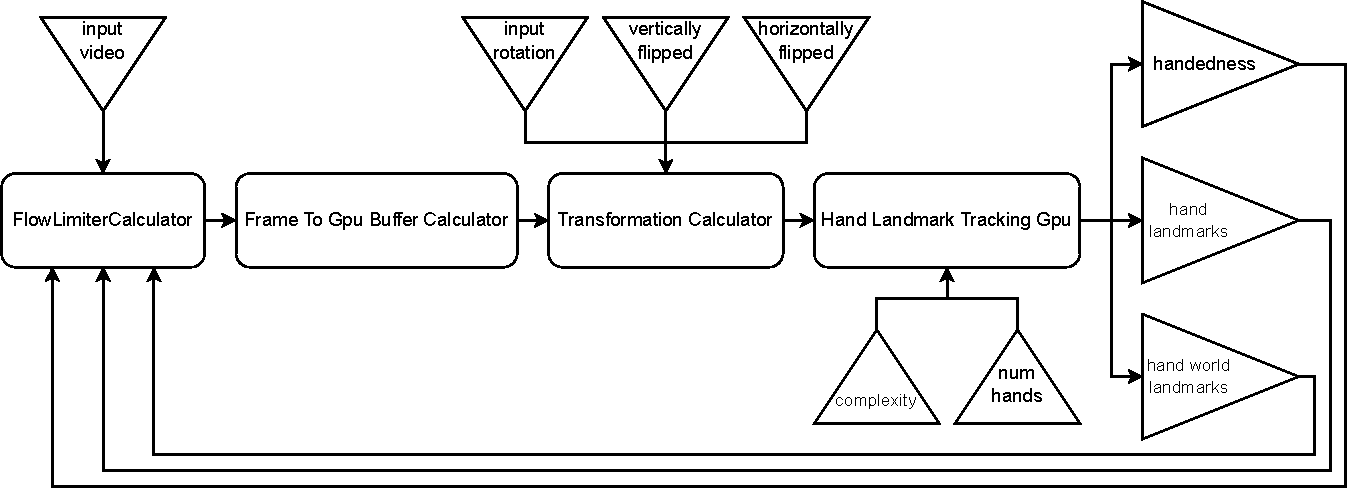
\includegraphics[width=\textwidth]{images/application/mediapipe-gpu}
	\caption{MediaPipe graph used in the application.}
	\label{fig:mediapipe-graph}
\end{figure}

The three data streams on which the outputs of the graph are passed work asynchronously
with respect to the main loop and also with respect to each other.
To ensure that the next step of the algorithm only starts when all three streams have produced a result
for the same frame, it was sufficient to implement a simple synchronisation system for the three outputs
to ensure that each frame is only passed to the next step of the algorithm when all three components are available.

Once all three components are available, our algorithm proceeds in its two phases:
\begin{itemize}
	\item \textit{Touch detection:} check if a finger touched the keyboard
	\item \textit{Note detection:} if a finger touched the keyboard,
	find which note was pressed and play the corresponding sound
\end{itemize}

It is important to note that, in its current state, not all three streams are used by our algorithm.
In particular, only the ones for \textit{hand landmarks} and \textit{handedness} are useful for our purposes.
The other, \textit{world hand landmarks}, is present mainly for reasons of compatibility with older
versions of the algorithm and the possibility that it will be useful in the future.

\paragraph{MediaPipe on low-end devices}
While the webcam and the video feed on the smartphone interface work at 30 FPS,
the frequency at which frames are sent to MediaPipe for hand detection is not fixed.
In order to meet all requirements and to be able to support as many smartphones as possible,
even low-end ones, we have implemented a way for the user to set the frequency at which frames are sent to
MediaPipe at will, i.e.\ the FPS at which the hand detection process runs.

This has been done by including buttons in the interface to directly increase and decrease the FPS with which to run MediaPipe.
Changing the value from the interface results in an immediate change in the operation of MediaPipe.

Through experimentation, we have found that a good value for MediaPipe's FPS is 15, which is high enough
to ensure that the app runs smoothly with low response times, but is not too high to be unusable on mid-range smartphones.

Going below 15 FPS is possible, but results in an increase in the app's response time and a possible loss of some notes.
Going above 15 FPS is also possible, and it is recommended in the case of high-end smartphones,
but being aware that increasing the frequency with which frames are sent to
MediaPipe also increases battery consumption and could lead to the smartphone overheating.

\subsubsection{Touch detection}
At this early stage of the project, the touch detection procedure is not yet very refined.
Since MediaPipe alone does not provide sufficiently precise depth coordinates (or camera distance) but rather
inconsistent and flickering ones, and for the reasons explained in \autoref{subsec:mp-for-3d}~\nameref{subsec:mp-for-3d},
we could not rely solely on them for the touch detection phase.
We therefore exploit the advantages explained in \autoref{subsec:pov}~\nameref{subsec:pov}.

To detect a touch, we rely on the position of the finger on the $y_s$ axis: when a finger reaches
down towards the paper to play a note, this movement is detected by MediaPipe thanks to the 45\degree \ view.
The $y_s$ position of the finger is given as input to an automaton that takes care
of maintaining and updating the state of the finger at each frame.
The automaton is illustrated in \autoref{fig:touch-automata}.

When a new frame is ready, the $x_s$ and $y_s$ positions of the finger are extracted from MediaPipe
and converted into pixels and the $y_s$ position is given to the automaton.
The automaton calculates the speed of the finger by comparing the new $y_s$ with the last detected $y_s$,
after which it advances the finger state accordingly.
When the finger enters the \textit{Touching} state, the $x_s$ and $y_s$ coordinates are passed to the note detector
which is responsible for verifying that the finger has touched a key and, if so, playing the corresponding note.
The automaton is made so that the \textit{Touching} state remains active even if the finger moves horizontally.

In \autoref{fig:touch-automata}, the \texttt{t} value indicates a threshold which serves to mitigate the instability of MediaPipe:
the hand landmarks detected by MediaPipe are subject to minute, continuous variations which, if not taken into account,
would cause a series of false positives and would repeatedly take the automaton in and out of the \textit{Touching} state.
Experimentally, we came to the conclusion that 8 is a suitable value for the automaton's activation threshold.

The pseudocode for this phase is shown in~\autoref{alg:touch-detection}.

\begin{algorithm}
	\caption{Touch detection}
	\begin{algorithmic}[1]
		\State when new frame arrives
		\If{no hand has been detected}
			\State \Return
		\EndIf
		\State $toPlay \gets \{\}$
		\For{each hand $h$ detected}
			\For{each finger $f$ of $h$}
				\State $x \gets$ horizontal position of $f$
				\State $y \gets$ vertical position of $f$
				\State $isPlaying \gets$ automata($f$).update($y$)
				\If{$isPlaying$}
					\State $toPlay \gets toPlay \ \bigcup \ \left\{ \left( x, y \right) \right\}$
				\EndIf
			\EndFor
		\EndFor
		\State do \textit{note detection} with $toPlay$
	\end{algorithmic}
	\label{alg:touch-detection}
\end{algorithm}

\begin{figure}[ht]
	\centering
	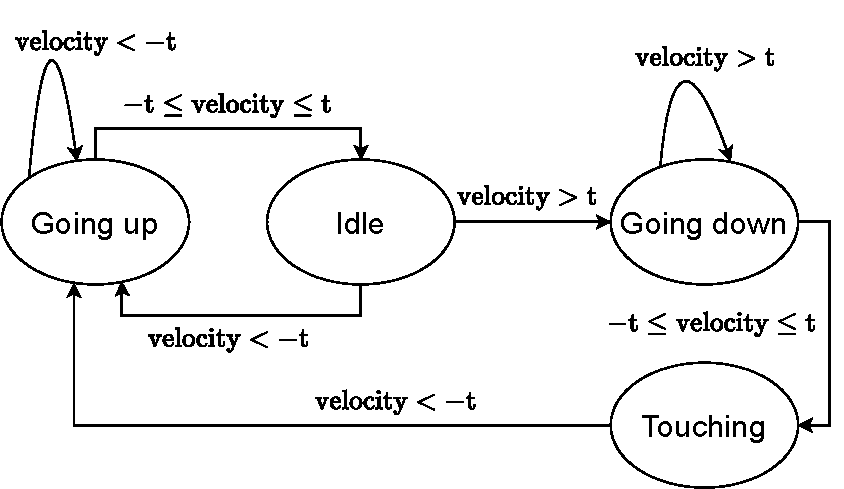
\includegraphics[width=\textwidth]{images/application/touch-automata}
	\caption{The automata used to detect finger touch.}
	\label{fig:touch-automata}
\end{figure}

\subsubsection{Note detection}\label{subsubsec:notes-detection}
Once we have detected the fingers touching the keyboard with MediaPipe,
we need to work out which notes have been touched.
To do this, we use the image generated in the keyboard detection phase in
\autoref{par:notes-detection}~\nameref{par:notes-detection}.

This image is the same size as the video feed and is totally black except where the keys are located.
The keys are coloured in a grey scale where the first key is coloured with the value 1,
the second with the value 2 and so on.
This allows us to associate each key with a unique value that we can use to determine the note to be played.

Using the $x_s$ and $y_s$ coordinates provided by MediaPipe, we can superimpose them on the image generated
in the keyboard detection phase to determine whether a finger has touched a key.
If the pixel at position $(x, y)$ is black, the finger is outside the keyboard and nothing happens.
If, on the other hand, the pixel is not black, the finger is on one of the detected keys and therefore the MIDI signal
corresponding to the detected note at that position must be played.

Playing sounds is not as straightforward a process as it might seem, and it does require a little forethought.
This is because when passing from one frame to another, some fingers that were playing
in the previous frame may still be playing the same key.
In this case the note does not have to be played again, but only continued.

To do this, we keep a list of the notes that are being played and, at each frame, create two different sets of notes:
the set of notes that were being played in the previous frame but are no longer being played in the current frame,
and the set of notes that were not being played in the previous frame but are being played in the current frame.

This allows to detect notes that were being played in the previous frame and are still being played in the current frame,
so that they are not played again but remain playing.

The pseudocode for this phase is shown in~\autoref{alg:note-detection}.

\begin{algorithm}
	\caption{Note detection}
	\begin{algorithmic}[1]
		\State \textbf{Input}: the set of coordinates $toPlay$ of the fingers touching the keyboard
		\State $playing \gets \{n \ | \ n \text{ is already being played from the previous frame}\}$
		\State $detected \gets \{ n \ | \ (x, y) \in toPlay \text{ and }\newline
		\hspace*{21.6mm} n \text{ is a non-black pixel at } (x, y) \text{ in the note image}\}$
		\State $stop \gets playing \setminus detected$
		\State $start \gets detected \setminus playing$
		\For{each $n$ in $stop$}
			\State stop playing note $n$
		\EndFor
		\For{each $n$ in $start$}
			\State start playing note $n$
		\EndFor
	\end{algorithmic}
	\label{alg:note-detection}
\end{algorithm}

\begin{figure}[ht]
	\centering
	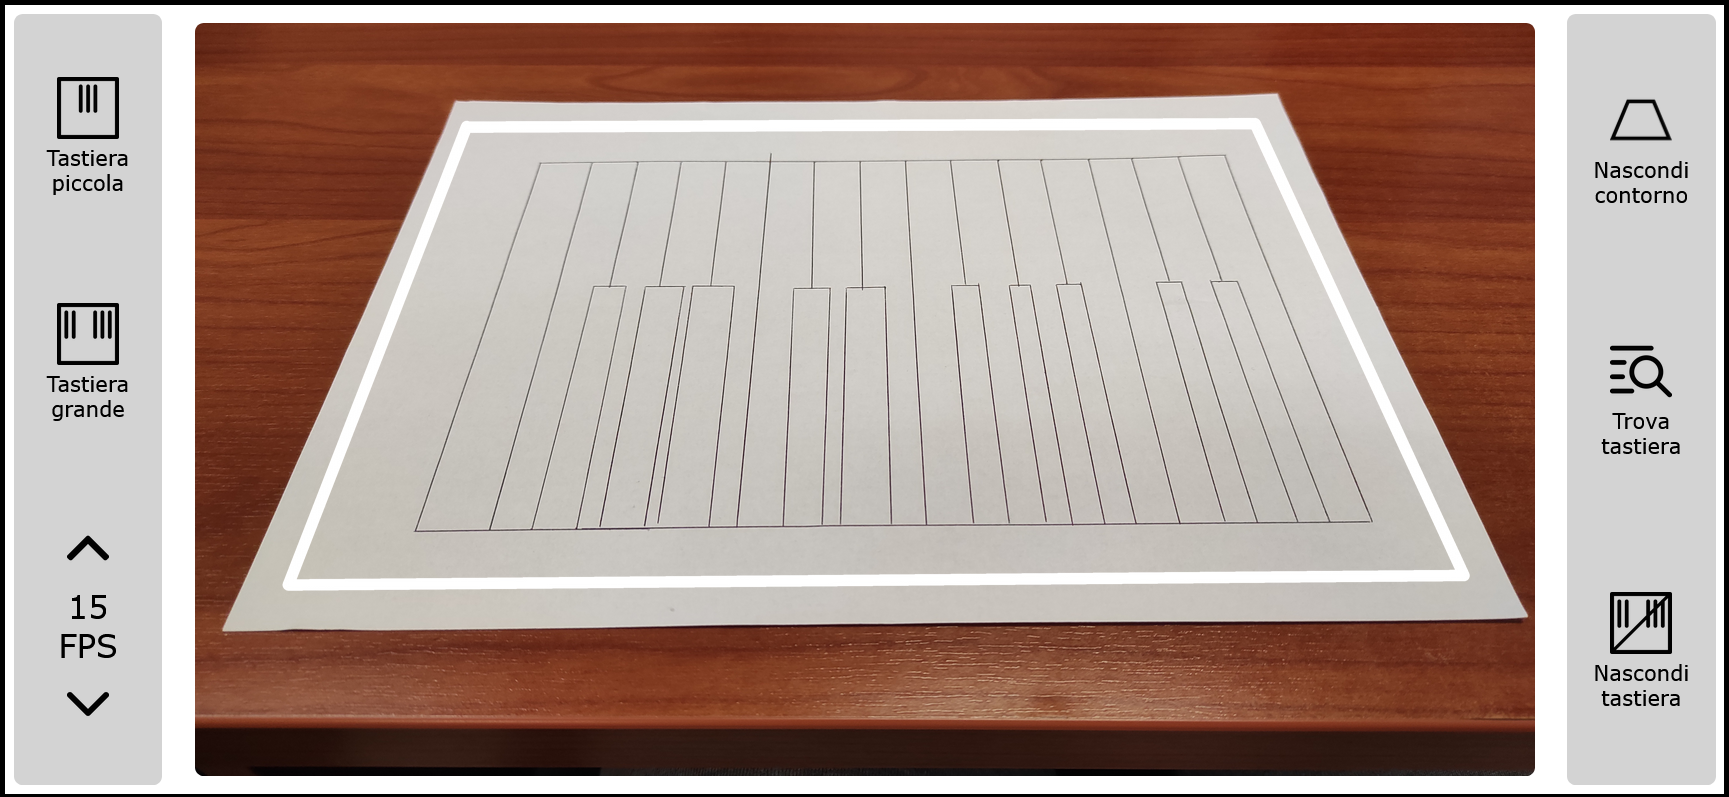
\includegraphics[width=\textwidth]{images/application/screenshots/detection-phase}
	\caption{Application during detection phase, with perimeter visible.}
	\label{fig:screenshot-detection-phase}
\end{figure}

\begin{figure}[ht]
	\centering
	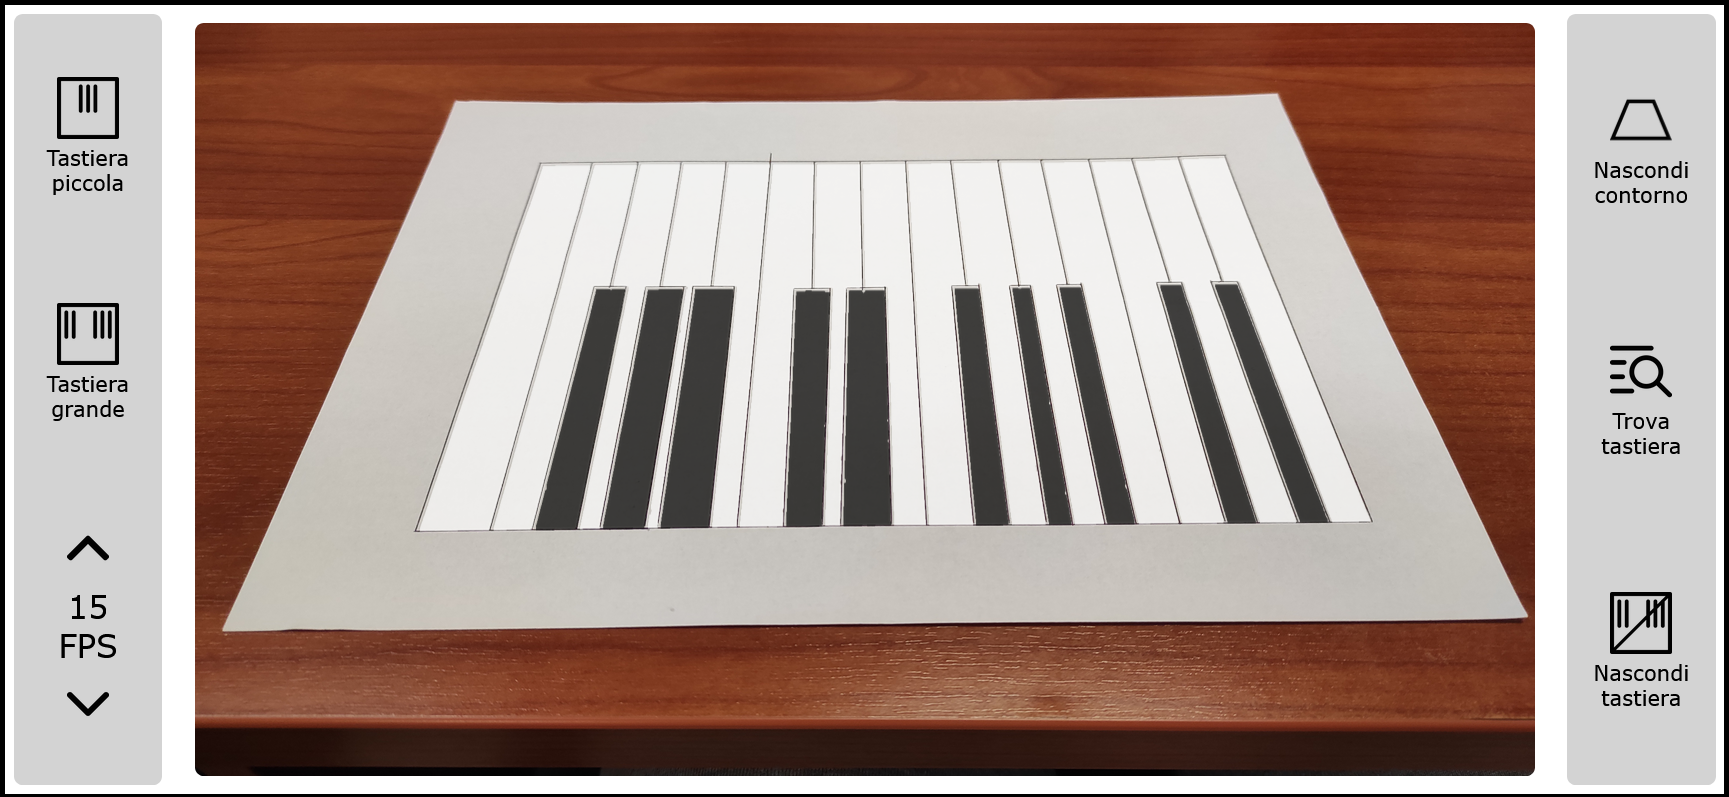
\includegraphics[width=\textwidth]{images/application/screenshots/playing-phase}
	\caption{Application after keyboard detection, with keyboard overlay visible.}
	\label{fig:screenshot-playing-phase}
\end{figure}
